\documentclass[11pt,a4paper]{article}
\usepackage[margin=0.6in]{geometry}
\usepackage[utf8]{inputenc}
\usepackage{hyperref}
\hypersetup{
    colorlinks=true,
    urlcolor=blue,
}
% package to make clickable, professional hyperlinks

\usepackage{amsmath, amsthm, amssymb, fancyhdr, pgfplots, enumerate, graphicx}

\pgfplotsset{compat=1.14}
\usepgfplotslibrary{fillbetween}

\newtheorem{theorem}{Theorem}
\newtheorem{lem}{Lemma}


\newcommand{\coursenum}{Crash Course Exercises}
\newcounter{problem}

\newcommand\Problem{
  \stepcounter{problem}
  {\large \textbf{Problem \theproblem.}~}
}

\fancyfoot[L]{Yang Gan}
\fancyfoot[C]{\small \LaTeX \ Exercises}
\fancyfoot[R]{\thepage}
\renewcommand\headrulewidth{0pt}
\pagestyle{fancy}

\begin{document}
\textbf{\coursenum \hfill}\\
\noindent\rule{\textwidth}{1pt} \\
\Problem \\\\
Replicate the following:\\\\
\noindent\rule{\textwidth}{.4pt} \\
\par
This is the start of a paragraph. This is some text 
\par
This is a new paragraph. \\\\
\textbf{No more indentation.}\\\\
On 25 June, 2020, the SPDR S\&P 500 ETF Trust closed at \$307.35. Here is a table of its \emph{most relevant} values:

\begin{center}
    \begin{tabular}{cc|cc}
        \textbf{Open} & 306.17 & \textbf{Div yield} & 1.91\% \\
        \hline 
        \textbf{High} & 306.39 & \textbf{Prev close} & 307.35 \\
        \hline 
        \textbf{Low} & 299.43 & \textbf{Mkt cap} & 268.01B
    \end{tabular}
\end{center}
As an exercise, attempt to figure out the following:
\begin{enumerate}[(i)]
\item
    Try to add ``Data from \emph{Google Finance}.'' as a caption below the table above. 
    
\item
    Attempt to re-align all the text above
    \begin{itemize}
        \item 
        Left align the first column
        \item
        Center align the second column
        \item
        Left align the third column
        \item
        Right align the last column
    \end{itemize}
\end{enumerate}

\pagebreak
\noindent\rule{\textwidth}{1pt} \\
\Problem \\\\
Replicate the following: \\
\noindent\rule{\textwidth}{.4pt} \\

\begin{enumerate}[a)]
\item
    \begin{align*}
        f'(x) &= \left(\frac{du}{dx}\right) \left( \frac{-\sin{u}}{\sqrt{1-\cos^2{u}}} \right) \\
        &= \frac{2}{1+x^2} \left( - \frac{2x}{1+x^2} \right) \left( \frac{1+x^2}{|2x|} \right) \tag{for $x\neq 0$}\\
        &= \sigma\left(\frac{2}{1+x^2}\right) 
    \end{align*}
    where
    \[ \sigma =\begin{cases}
                    -1 & \text{ for } x>0\\
                    1  & \text{ for } x<0
                \end{cases}
    \]
    Our domain will hence be $(-\infty, 0) \cup (0, \infty)$. Note that
    \[
        y_x \in \mathbb{R} \iff y_x < \frac{\pi}{2}
    \]

\item
    The characteristic polynomial is
    \begin{align*}
        \det \begin{bmatrix}
            3 - \lambda & -1 \\
            1 & 1 - \lambda
        \end{bmatrix} &= (3 - \lambda)(1 - \lambda) - (-1)(1) \\
        &= \lambda^2 - 4\lambda + 4 \\
        &= (\lambda - 2)^2
      \end{align*}
      As such,
      \[
        \lambda_1 = \lambda_2 = 2
      \]

\item
    We have
    \begin{theorem}[Wave Equation Solution]
    \begin{align*}
        u(x, t) =  \sum_{n = 1}^\infty \Big[ &A_n \sin\left(\frac{n\pi x}{L} \right) \cos\left(\frac{n\pi \alpha t}{L} \right) \\
        + &B_n \sin\left(\frac{n\pi x}{L} \right) \sin \left(\frac{n\pi \alpha t}{L} \right)\Big] \tag{1}
    \end{align*}
    Where
    \begin{align*}
        A_n &= \frac{2}{L}\int_0^L f(x) \sin\left(\frac{n\pi x}{L} \right) dx \\
        B_n &= \frac{2}{n\pi \alpha}\int_0^L g(x) \sin\left(\frac{n\pi x}{L} \right) dx
    \end{align*}
    \begin{proof}
        By observation.
    \end{proof}
    \end{theorem}
\end{enumerate}

\pagebreak
\noindent\rule{\textwidth}{1pt} \\
\Problem \\\\
Replicate the following: \\
\noindent\rule{\textwidth}{.4pt} \\\\
We want to plot the following function:
\[
    f(x) = \begin{cases}
        (x^8+x^{16})/(1+x^{24}) & \text{  for $0 \leq x < 1$} \\
        0 & \text{  for $x = 1$}
    \end{cases}
\]First we use \href{https://www.desmos.com/calculator/t6htfjnive}{Desmos}

\begin{figure}[hbt]
    \centering
    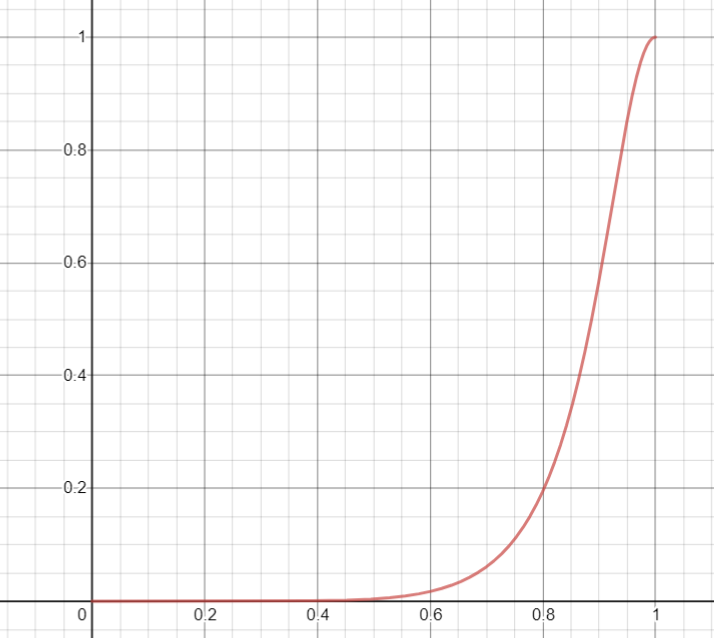
\includegraphics[width=.6\linewidth]{desmos.PNG}
    \caption{Demos graph of $f(x)$}
\end{figure}

Next, we use pgfplots:

\begin{figure}[h]
    \centering
    \begin{tikzpicture}
        \begin{axis}[
        width=\textwidth/1.5,
        height=\axisdefaultheight,
        axis x line=center,
        axis y line=left,
        xtick={0, 1},
        xticklabels={$0$, $1$},
        ytick={0, 1},
        yticklabels={$0$, $1$},
        xlabel={$x$},
        ylabel={$f(x)$},
        xlabel style={right},
        ylabel style={above},
        xmin= 0,
        xmax= 1.3,
        ymin=-0.2,
        ymax= 1.3]
        \addplot [
            domain = 0:1,
            samples = 100,
        ] {(x^8+x^16)/(1+x^24)};
        \addplot[only marks, mark=*, mark options={fill=white}]
        coordinates {(1, 1)};
        \addplot[only marks, mark=*, mark options={fill=black}]
        coordinates {(1, 0)};
        \end{axis}
    \end{tikzpicture}
    \caption{Pgfplots graph of $f(x)$}
\end{figure}

\end{document}